\documentclass[12pt, a4paper]{article}

\usepackage{fancyhdr}
\usepackage[left=4cm, right=4cm, top=4cm, bottom=4cm]{geometry}
\usepackage[utf8]{inputenc}
\usepackage[table]{xcolor}
\usepackage{hyperref}
\usepackage{amsmath}
\usepackage{enumitem}
\usepackage{graphicx}
\usepackage{booktabs}
\usepackage{subcaption}
\usepackage[justification=centering]{caption}
\usepackage{xepersian}

\DeclareMathOperator*{\argmax}{argmax}
\DeclareMathOperator*{\argmin}{argmin}
\newcolumntype{L}{>{$}l<{$}} % math-mode version of "l" column type

\newcommand{\coursetitle}{شبکه‌های عصبی}
\newcommand{\doctitle}{تمرین دوم}
\newcommand{\name}{محمدرضا غفرانی}
\newcommand{\studentno}{400131076}
\newcommand{\todaydate}{\today}

\settextfont{XB Kayhan}
\setlatintextfont{Times Newer Roman}

\pagestyle{fancy}
\lhead{\textbf{\doctitle}}
\chead{\name}
\rhead{\todaydate}

\begin{document}

\begin{flushleft}
    \name \\
    \studentno \\
    \todaydate
\end{flushleft}

\begin{center}
    \huge
    \textbf{\coursetitle}
    \break
    \large
    \doctitle
\end{center}

% suppress the fancy header on the first page only
\thispagestyle{plain}

\section*{سوال یک}

با استفاده از الگوریتم‌های خوشه‌بندی می‌توان ابعاد داده‌ها را کاهش داد. برای انجام این کار دو راه داریم یکی این که
بعد از انجام خوشه‌بندی هر داده را با فاصله آن از مراکز خوشه نشان دهیم. دو این که
هر داده را با شناسه خوشه‌اش نشان دهیم. برای توضیح بهتر از مثال کمک می‌گیریم، فرض کنید که بخواهیم داده‌ها را از
فضای ۱۰۰ بعدی به فضای با ابعاد پایین‌تر نگاشت کنیم. در این حالت بعد از انجام عمل خوشه‌بندی
۲ راه در پیش داریم. داده‌ها را با فاصله آن داده از مراکز خوشه‌ها نمایش دهیم. در این حالت اگر ۴ خوشه داشته باشیم،
داده‌ها از فضای ۱۰۰ بعدی به فضای ۴ بعدی نگاشت می‌شود. در روش دوم به داده هر خوشه یک عدد نسبت داده و هر عضو آن خوشه را با
عدد نمایش می‌دهیم. بدین ترتیب ما از فضای ۱۰۰ بعدی به فضای یک بعدی نگاشت کرده‌ایم.
از آن جا که شبکه‌های کوهونن نیز نوعی از الگوریتم‌های خوشه‌بندی هستند بنابراین به شیوه مشابهی عمل می‌کنیم.
این شبکه‌ لایه پنهان نداشته و صرفا شامل لایه ورودی و خروجی است.
الگوریتم یادگیری این شبکه‌ها اصطلاحا رقابتی نامیده می‌‌شود. این نام‌گذاری از شیوه عملکرد این شبکه نشئت می‌گیرد.
با اعمال ورودی و تولید خروجی‌ها بررسی می‌شود که کدام نورون نسبت به باقی نورون‌ها به ورودی شبکه
نزدیک‌تر است. با مشخص‌شدن نزدیک‌ترین نورون به ورودی، آن نورون اصطلاحا برنده شده و وزن‌های آن و
یک همسایگی مشخصی از نورون‌های اطراف به‌روز می‌شود. با ادامه این روند در گام‌های بعد وزن‌ نورون‌ها تغییر کرده و
شبکه ساختار کلی داده‌ها را به خود می‌گیرد. حال اگر بخواهیم داده‌ها را با فاصله آن از مراکز خوشه‌ها نشان دهیم
ابعاد جدید داده‌ها برابر تعداد نورون‌های موجود در لایه خروجی خواهد بود. اما اگر بخواهیم هر داده را با شناسه
نورونی که به آن نسبت داده شده است نمایش دهیم، در این حالت فضایی که به آن نگاشت می‌شود متناسب با ساختار
قرارگیری نورون‌های خروجی خواهد بود. بدین معنی که اگر نورون‌ها به صورت خطی پشت سر هم گذاشته شده باشند،
از آن جا که شناسه نسبت داده شده به آن‌ها یک عدد است داده‌ها به فضای یک بعدی، و اگر نورون‌ها در یک صفحه باشند،
به دلیل آن که شناسه هر نورون یک زوج مرتب دو بعدی است، بنابراین داده‌ها به فضای دو بعدی منتقل خواهند شد.

\section*{سوال دو}

منظور از نورون مرده در شبکه خودسامانده کوهونن، نورونی است که به دلیل دور بودن وزن‌های آن از ورودی‌های اولیه
هیچ‌گاه در رقابت برنده نمی‌شود. در این شبکه‌ها تنها وزن نورون‌هایی تغییر می‌کند که در رقابت برنده شوند،
بنابراین توضیح وزن نورون‌های مرده تنها ممکن است به دلیل به‌روزرسانی وزن یکی از همسایه‌ها تغییر کند،
در غیر این صورت همواره ثابت باقی می‌ماند. وجود این نورون‌ها به‌خودی‌خود بد نیستند، اما از آن جا که هیچ
داده‌ای به آن‌ها نسبت داده نمی‌شود بنابراین بی‌جهت توانایی عمل را از مدل گرفته و اجازه نمی‌دهند شبکه بتواند یک
خوشه‌بندی بهتری را از داده‌ها ارائه دهد.

برای رفع این مشکل می‌توانیم وزن‌های اولیه نورون‌ها از داده‌های ورودی انتخاب کنیم، بدین ترتیب هر نورون می‌تواند
حداقل به ازای یک داده برنده شده و شانس تغییر داشته باشد. روش دیگری که برای حل این مشکل به نظر می‌رسد،
ایده برداری از الگوریتم‌هایی نظیر \lr{Kmeans++} است. این الگوریتم برای مقداردهی اولیه مراکز خوشه در الگوریتم
\lr{Kmeans} استفاده می‌شود. در این الگوریتم مراکز اولیه از بین داده‌ها انتخاب می‌شود، اما برای آن که
به حداکثر کارآیی برسیم پس از انتخاب یک داده به عنوان مرکز خوشه، دورترین داده از داده فعلی برای مرکز خوشه دوم
انتخاب می‌شود. در این جا نیز می‌توانیم در هنگام مقدار اولیه وزن‌ها از روی داده‌ها، داده‌هایی که بیشترین فاصله از هم
را دارند را انتخاب کنیم تا شانس این که هر داده‌ها به صورت یکنواخت بین نورون‌ها توزیع شوند بیشتر شود.

\section*{سوال سه}

مجموعه داده \lr{human activity recognition using smartphones} خود داده‌های آموزش و آزمون را از هم تفکیک کرده است.
این تفکیک به نسبت ۷ به ۳ صورت گرفته یعنی حدود ۷۰ درصد داده‌ها به عنوان داده آموزشی و ۳۰ داده‌ها به عنوان داده
آزمون فرض شده است. اما با توجه به صورت تمرین داده‌ها باید به نسبت ۷-۲-۱ بین داده‌های آموزش، ارزیابی و آزمون تقسیم شود.
با توجه به آن که در حال حاضر خود مجموعه داده، ۷۰ درصد داده‌های آموزشی را به عنوان داده آموزشی در نظر گرفته است؛
بنابراین تصمیم گرفتیم داده‌های ارزیابی را از مجموعه داده تست انتخاب کنم.
بنابراین ۷۰ درصد مجموعه داده آزمون را به عنوان مجموعه داده ارزیابی و باقی را به عنوان داده آزمون استفاده کردیم.

\section*{سوال چهار}

ساختار کلی شبکه عصبی چندلایه پرسپترونی که در این تمرین استفاده شده است، در شکل \ref{mlp} دیده می‌شود.
از آن جا که همه ورودی‌ها به صورت عددی بوده و در بازه
$(-1,1)$ قرار دارند، بنابراین پیش‌پردازش خاصی بر روی داده‌ها انجام نمی‌دهیم.
ساختار کلی شبکه عصبی ارائه شده به صورت موجود در شکل زیر است.

\begin{figure}[h]
    \centering
    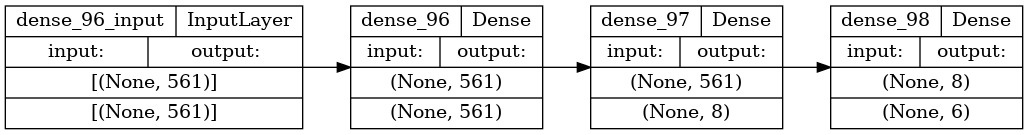
\includegraphics[width=0.8\linewidth]{images/mlp.png}
    \caption{معماری کلی شبکه پرسپترونی چندلایه مورد استفاده}
    \label{mlp}
\end{figure}

برچسبی که به هر نمونه آموزشی در مجموعه دادگان داده شده است، عددی بین یک تا ۶ است. با توجه به عملکرد بسیار مناسب
کدگذاری \lr{one-hot} و کوچک بودن بردار نسبت داده شده توسط این کدگذاری برای هر نمونه، بنابراین ما برچسب دادگان را
به کدگذاری \lr{one-hot} تغییر می‌دهیم.

ما آزمون خطاهای زیر را برای یافتن تعداد بهینه لایه‌ها و تعداد نورون موجود در هر لایه بررسی کرده‌ایم.
از آن جا که در دفعات مختلف آموزش، شبکه عملکرد متفاوتی را از خود نشان می‌داد؛ بنابراین ما چند بار
شبکه‌های عصبی را بر روی داده‌های آموزشی آموزش داده و در نهایت بهترین عملکرد شبکه را گزارش می‌کنیم.
در هنگام انجام این آزمایشات ما از بهینه‌ساز \lr{Adams} با نرخ یادگیری ثابت $0.0001$ در نظر گرفتیم.
نتایج عملکرد شبکه در جدول \ref{mlp_performance} دیده می‌شود.

\begin{latin}
\begin{table}[!ht]
    \centering
    \caption{\rl{آزمون خطاهای انجام شده برای یافتن تعداد بهینه لایه‌های پنهان و نورون‌ها}}
    \label{mlp_performance}
    \begin{tabular}{|l|l|c|c|c|c|}
    \hline
        & & \multicolumn{2}{c|}{train} & \multicolumn{2}{c|}{validation}  \\ \hline
        index & hidden layer & accuracy & loss & accuracy & loss \\ \hline
        1 & - & 0.9064 & 0.3465 & 0.9049 & 0.3775 \\ \hline
        2 & (8,) & 0.9446 & 0.2392 & 0.9108 & 0.2999 \\ \hline
        3 & (8,8) & 0.9132 & 0.416 & 0.8676 & 0.4607 \\ \hline
        4 & (8,8,8) & 0.565 & 0.8213 & 0.5674 & 0.8799 \\ \hline
        5 & (32,) & 0.9642 & 0.1263 & 0.9394 & 0.1857 \\ \hline
        6 & (64,) & 0.9676 & 0.1099 & 0.9462 & 0.167 \\ \hline
        7 & (128,) & 0.9716 & 0.0906 & 0.9442 & 0.1656 \\ \hline
        8 & (256,) & 0.9771 & 0.0773 & 0.9491 & 0.1454 \\ \hline
        9 & (512,) & 0.978 & 0.0703 & 0.9486 & 0.1452 \\ \hline
        10 & (1024,) & 0.9819 & 0.0596 & 0.9467 & 0.1538 \\ \hline
        11 & (2048,) & 0.9839 & 0.0511 & 0.9525 & 0.1371 \\ \hline
        12 & (4096,) & 0.9864 & 0.0444 & 0.9433 & 0.1549 \\ \hline
        13 & (8192,) & 0.9886 & 0.0382 & 0.9515 & 0.1391 \\ \hline
        14 & (8192, 8192) & 0.9967 & 0.0119 & 0.9496 & 0.1904 \\ \hline
        15 & (8192, 8192, 8192) & 0.9967 & 0.0096 & 0.9486 & 0.2062 \\ \hline
        16 & (4096, 4096, 4096, 4096) & 0.9962 & 0.0105 & 0.951 & 0.1875 \\ \hline
    \end{tabular}
\end{table}
\end{latin}

با توجه به این نتیجه هر چقدر تعداد لایه‌ها و تعداد نورون‌های موجود در هر لایه بیشتر باشد
عملکرد شبکه بهتر می‌شود. ما شبکه آموزش دیده با مشخصات $(4096, 4096, 4096, 4096)$ را به علت
کم بودن نرخ \lr{loss} آن از دیگر مدل‌ها با وجود ارائه صحت برابر، انتخاب کرده و از این
پس نتایج را با آن گزارش می‌کنیم. در ادامه با آزمون و خطا سعی می‌کنیم بهترین مقدار نرخ یادگیری
را برای این شبکه پیدا کنیم. در این حالت نیز مدل را چند‌بار اجرا کرده و بهترین عملکرد آن‌ را گزارش می‌دهیم.
با توجه به جدول \ref{mlp_learning_rate}  مدل در هنگامی که نرخ یادگیری برابر $0.0001$
بهترین عملکرد را از خود نشان می‌دهد، در نتیجه ما در ادامه از این نرخ یادگیری برای ارائه نتایج استفاده خواهیم کرد.
عملکرد این شبکه در داده‌های آزمون از نظر معیار‌های صحت و خطا به ترتیب برابر $0.9695$ و $0.1077$ است.

\begin{latin}
\begin{table}[!ht]
    \centering
    \caption{\rl{آزمون خطاهای انجام شده برای یافتن بهترین نرخ یادگیری}}
    \label{mlp_learning_rate}
    \begin{tabular}{|l|l|c|c|c|c|}
    \hline
        & & \multicolumn{2}{c|}{train} & \multicolumn{2}{c|}{validation}  \\ \hline
        index & learning rate & accuracy & loss & accuracy & loss \\ \hline
        1 & 1E-06 & 0.8823 & 0.4845 & 0.8657 & 0.5149 \\ \hline
        2 & 1E-05 & 0.9864 & 0.0458 & 0.9457 & 0.1341 \\ \hline
        3 & 0.0001 & 0.9958 & 0.0117 & 0.9437 & 0.1924 \\ \hline
        4 & 0.001 & 0.9848 & 0.038 & 0.9437 & 0.2092 \\ \hline
        5 & 0.01 & 0.9457 & 0.14 & 0.9006 & 0.2867 \\ \hline
        6 & 0.1 & 0.184 & 1.7843 & 0.1765 & 1.7901 \\ \hline
    \end{tabular}
\end{table}
\end{latin}

\newpage

با توجه به آزمون خطاهای انجام شده اگر ما مدلی با سه لایه مخفی که هر یک 4096 نورون دارد را انتخاب می‌کنیم،
مدل بهترین عملکرد را از خود نشان می‌دهد. با تنظیم نرخ یادگیری
بر روی مقدار ثابت $0.0001$ مدل پیشنهادی می‌تواند به صحت ۹۹ درصد برسد که نتیجه بسیار خوبی است.

\section*{سوال پنجم}

در ابتدا توضیحاتی در رابطه با جزئیات پیاده‌سازی شبکه خودسامانده کوهونن داده شده و سپس تاثیر تغییر پارامتر‌های مختلف
را بر روی عملکرد آن را بررسی می‌کنیم.

شبکه خودسامانده پیاده‌سازی شده از یک لایه ورودی و یک لایه خروجی تشکیل شده است. تعداد نورون‌های موجود در لایه خروجی
جزو پارامتر‌های مسئله بوده و ما در ادامه با تغییر آن تلاش خواهیم کرد بهترین خوشه‌بندی را برای داده‌ها پیدا کنیم
اما شیوه قرار گرفتن نورون‌های خروجی همواره به صورت دو بعدی است. تعداد نورون‌های موجود در لایه ورودی نیز برابر تعداد
ویژگی‌های داده‌ها و برابر ۵۶۱ است. در هنگام آموزش نرخ یادگیری به صورت خطی با فرمول زیر کاهش می‌یابد.

$$lr = lr_0 - \alpha \times t$$

منظور از $lr_0$ نرخ یادگیری اولیه، منظور از $\alpha$ شیب نرخ کاهش یادگیری و
منظور از $t$ گام یادگیری متناظر محاسبه $lr$ است. در این پیاده‌سازی شعاع اثر نورون‌ برنده
همواره ثابت است. میزان اثر این نورون به همسایه‌های مجاور آن با فرمول $\frac{1}{d+1}$ محاسبه می‌شود که منظور از $d$
فاصله اقلیدسی نورون مدنظر از نورون برنده است. همسایگی نورون‌ها از یکدیگر به صورت دایره‌ای در نظر گرفته شده است.
همچنین وزن‌ها در ابتدا از میان داده‌ها و به صورت تصادفی انتخاب شده‌اند. در شکل \ref{som_performance}
یک نمونه از خوشه‌بندی انجام شده در ابتدای یادگیری و خوشه‌بندی نهایی آورده می‌شود. همان‌طور که مشاهده می‌شود
شبکه \lr{SOM} توانسته‌ است الگوی کلی داده‌ها را شناسایی کرده و آن‌ها را از یکدیگر تمییز دهد.

\begin{figure}[h]
    \centering
    \begin{subfigure}{0.8\linewidth}
        \centering
        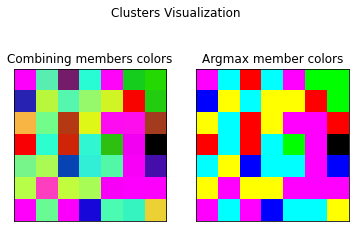
\includegraphics[width=0.8\linewidth]{images/som_example/initial.png}
        \caption{خوشه‌بندی اولیه}
    \end{subfigure}
    \begin{subfigure}{0.8\linewidth}
        \centering
        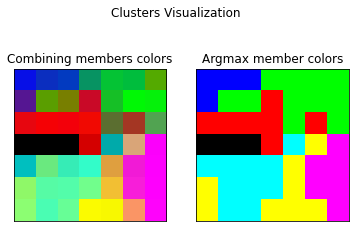
\includegraphics[width=0.8\linewidth]{images/som_example/final.png}
        \caption{خوشه‌بندی نهایی}
    \end{subfigure}
    \caption{}
    \label{som_performance}
\end{figure}

حال که جزئیات پیاده‌ساده شبکه را بررسی کردیم، عملکرد شبکه را به ازای تغییر پارامتر‌های مختلف آن بررسی می‌کنیم.
در شکل‌های \ref{r1} تا \ref{r18} عملکرد شبکه به ازای پارامتر‌های مختلف دیده می‌شود.
به ازای هر پارامتر شش نمودار رسم شده است. مفهوم بیشتر نمودار‌ها
با توضیح مختصری که به صورت «عنوان» آورده شده است، مشخص بوده و نیاز به توضیح اضافی ندارد.
با این حال ارائه توضیحاتی برای دو نمودار که در بخش (آ) هر شکل رسم شده است، ضروری به نظر می‌رسد.
به صورت خلاصه این دو نمودار توزیع کلی برچسب‌ها در بین نورون‌های مختلف را نشان می‌دهند.
نمودار \lr{Argmax} به هر نورون برچسب داده‌ای که بیشترین تکرار را دارد نسبت می‌دهد اما در نمودار دوم میانگین برچسب
داده‌هایی که به آن نورون نزدیک‌ترین هستند، محاسبه شده و سپس رنگ متناظر به آن نسبت داده می‌شود. در نمودار \lr{U-Matrix}
نیز توزیع داده‌ها در بین نورون‌های مختلف خروجی آورده شده است. نقاط قرمز پررنگ توزیع بیشتر و نقاط سفید‌تر توزیع کم‌تر را
نشان می‌دهند. نکته دیگری که لازم به توضیح است در این جا فرض شده است نورون‌ مرده نورونی است که در یک گام یادگیری
برنده نشده است. این تعریف اندکی با تعریف اصلی نورون مرده که نورون مرده نورونی است که هیچگاه در طی یادگیری
برنده نشوند متفاوت است. چون در طی آموزش تمامی نورون‌ها حداقل یکبار برنده می‌شدند بنابراین تعریف نورون مرده را
بدین شکل در نظر گرفتیم.

حال تاثیر هر پارامتر را بر روی خروجی هر نورون بررسی می‌کنیم. اولین پارامتری مورد بررسی پارامتر ابعاد نقشه است.
ما عملکرد شبکه را به ازای ابعاد نقشه $5 \times 5$، $7 \times 7$، $10 \times 10$ و $13 \times 13$ بررسی کرده‌ایم.
با افزایش ابعاد نقشه مدل آزادی عمل مدل بیشتر شده و در نتیجه قدرت مدل در جداسازی ‌خوشه‌های مختلف از هم بهتر می‌شود.
برای مثال دو شکل \ref{r2} و \ref{r15} را در نظر بگیرید. در شکل \ref{r2} خوشه‌ها تقریبا هیچ فاصله‌ای از یکدیگر ندارند
اما در شکل \ref{r15} دادهای مربوط به یک دسته در بین نورون‌های مختلف پخش شده است. این حالت باعث می‌شود جدا کردن دسته‌‌های
مختلف از هم ساده‌تر باشد کما این که در \lr{U-Matrix} شکل \ref{r15} توزیع داده‌ها در بین خوشه‌های مختلف به وضوح از
فاصله دارد و در نتیجه جدا کردن داده‌ها در این حالت راحت‌تر است. زیاد بودن تعداد نورون‌ها در حالت \ref{r15} از جنبه
زیاد بودن تعداد نورون‌های مرده نیز قابل بررسی است. در حالت \ref{r2} به علت کم‌بودن تعداد نورون‌ها و در نتیجه کم‌بودن
رقابت بین آن‌ها، هیچ نورونی بدون عضو باقی نمانده است. البته ایجاد نورون‌های مرده علاوه بر این پارامتر تابع پارامترهای
دیگر نیز هست که در ادامه بررسی خواهد شد. در حالت کلی با افزایش ابعاد نقشه به دلیل زیاد شدن
تعداد نورون‌ها احتمال این که یک نورون از رقابت جا مانده و داده‌ها به نورون دیگر نسبت داده شود بیشتر می‌شود. این مسئله در
شکل‌ها نیز مشخص است. نکته دیگری که در هنگام افزایش ابعاد مدل قابل مشاهده است کم شدن فاصله نورون
برنده از داده‌های عضو آن خوشه است. در حالت حدی هر نورون نماینده یک داده بوده
و در نتیجه فاصله آن از داده منتسب به آن برابر صفر خواهد بود.

نرخ یادگیری سرعت حرکت مدل به حالت بهینه را تعیین می‌کند. اگر میزان این پارامتر زیاد باشد شاهد تغییرات زیاد در
وزن‌ها و میانگین فاصله نورون‌های برتر خواهیم بود. در پیاده‌سازی انجام شده نرخ یادگیری به صورت خطی با شیب $\alpha$ کاهش پیدا می‌کند.
هر چقدر میزان پارامتر $\alpha$ کم‌تر باشد نرخ یادگیری با سرعت کم‌تری کاهش یافته و در نتیجه در طول آموزش عدد بزرگتری است.
با انتخاب مقادیر بزرگ برای نرخ یادگیری، تغییرات وزن‌ها بیشتر بوده و در نتیجه نمودار شبکه دارای نوسانات بیشتری است.
برای مثال نتایج حاصل شده در شکل‌های \ref{r10}، \ref{r11} و \ref{r12} را در نظر بگیرید. در این شکل‌ها سایر پارامتر‌ها
ثابت است اما میزان پارامتر $\alpha$ رفته‌رفته بیشتر شده است. همان‌طور که مشاهده می‌شود فاصله نورون برنده در حالتی
که $\alpha=0.005$ است با روند بسیار آرام‌تری نسبت به دو حالت دیگر کاهش یافته است. شدید بودن تغییرات در نمودار
تغییر وزن‌ها نیز قابل مشاهده است. در همین مثال در حالتی که $\alpha=0.005$ است میزان تغییرات وزن نورون‌ها بسیار
آرام‌تر از دو حالت دیگر است. در حالتی که $\alpha$ بزرگ است به دلیل تغییرات زیاد ممکن است در هنگام اتمام آموزش
خوشه‌بندی انجام شده در حالت مناسب نبوده و در نتیجه نتواند یک بازنمایی درستی ارائه دهد.

پارامتر تاثیرگذار بعدی، شعاع همسایگی است. هر چقدر شعاع همسایگی بیشتر باشد نورون‌ برنده به همسایه‌های بیشتری تاثیر‌
می‌گذارد. به همین دلیل در حالت‌هایی که شعاع همسایگی بالایی دارند، خوشه‌ها در گوشه‌های شکل تجمع یافته‌اند، چرا که
نورون‌های موجود در گوشه، هم زمانی که خود در رقابت برنده می‌شوند به‌روز‌ می‌شوند و هم زمانی که نورون‌های مرکزی برنده می‌شوند،
به دلیل همین اتفاق خوشه‌ها معمولا در نقاط کناری شکل تشکیل می‌شوند. برای مثال شکل‌های
\ref{r9} و \ref{r14} را در نظر بگیرد. در این دو شکل به دلیل زیاد بودن شعاع همسایگی دو داده‌ها به دو دسته‌ تقسیم شده‌اند.
مثلا در شکل \ref{r9} یک قسمت زیادی از داده‌ها در یک گوشه و قسمت دیگر در گوشه مقابل تجمع کرده‌اند. البته در این حالت
نیز خوشه‌بندی بین دسته‌ها تا جای ممکن انجام شده است.

با توجه به توضیحات بالا به نظر می‌رسد شبکه موجود در شکل‌ \ref{r17} بهترین عملکرد را داراست. چرا که تقریبا
هر نورون خروجی شبکه \lr{SOM} نمایندگی تنها یک دسته از داده‌ها را به عهده داشته و در نتیجه خوشه‌ها تقریبا خالص هستند.
این موضوع از روی شکل خوشه‌بندی و مقایسه بین خوشه‌بندی در حالتی که رنگ نورون به صورت \lr{Argmax} با زمانی که رنگ
نورون به صورت ترکیبی از رنگ اعضای آن نشان داده می‌شود قابل برداشت است. بعلاوه در این شکل‌ نمودار \lr{U-Matrix}
با نمودار خوشه‌بندی هماهنگ بوده و در نتیجه می‌توان این استنباط را داشت که هر خوشه خلوص بالایی دارد.

\clearpage

\begin{figure}[h]
    \begin{subfigure}{\linewidth}
        \centering
        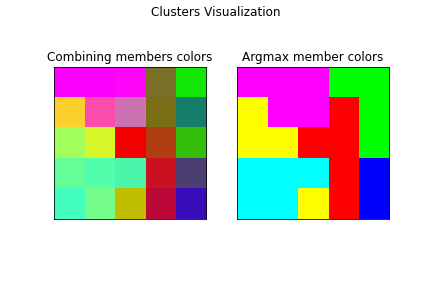
\includegraphics[width=0.8\linewidth]{images/q5/r1/cluster.png}
        \caption{خوشه‌بندی انجام شده توسط شبکه خودسامانده}
    \end{subfigure}
    \newline
    \begin{subfigure}{0.45\linewidth}
        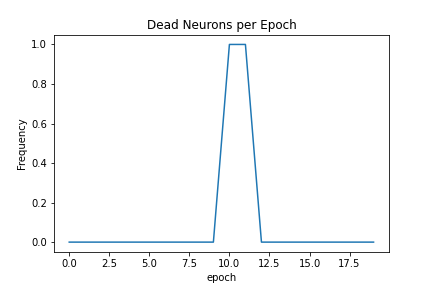
\includegraphics[width=\linewidth]{images/q5/r1/dead.png}
        \caption{تعداد نورون‌های مرده در هر گام}
    \end{subfigure}
    \hfill
    \begin{subfigure}{0.45\linewidth}
        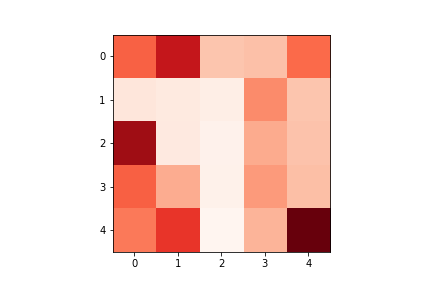
\includegraphics[width=\linewidth]{images/q5/r1/umatrix.png}
        \caption{نمودار \lr{U-Matrix}}
    \end{subfigure}
    \newline
    \begin{subfigure}{0.45\linewidth}
        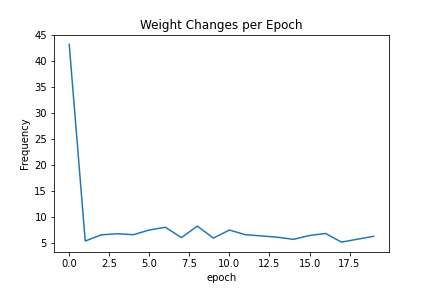
\includegraphics[width=\linewidth]{images/q5/r1/weight_change.png}
        \caption{تغییر وزن‌ها در هر گام}
    \end{subfigure}
    \hfill
    \begin{subfigure}{0.45\linewidth}
        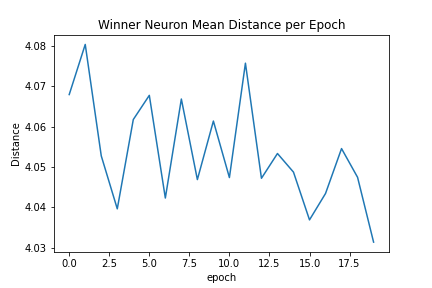
\includegraphics[width=\linewidth]{images/q5/r1/winner_distance.png}
        \caption{فاصله نورون برنده از نورون مدنظر در یک گام}
    \end{subfigure}
    \caption{نمودار‌های آموزش شبکه \lr{SOM} با پارامتر‌های \\$R=2$, $\alpha=0.001$ و ابعاد نقشه $5 \times 5$ با $lr_0=0.1$ و $T=10$}
    \label{r1}
\end{figure}

\clearpage

\begin{figure}[h]
    \begin{subfigure}{\linewidth}
        \centering
        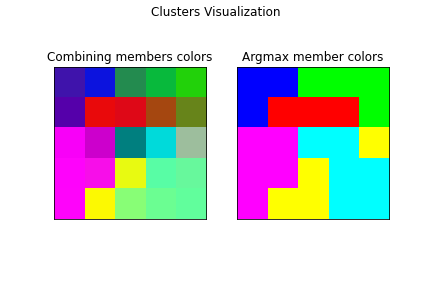
\includegraphics[width=0.8\linewidth]{images/q5/r2/cluster.png}
        \caption{خوشه‌بندی انجام شده توسط شبکه خودسامانده}
    \end{subfigure}
    \newline
    \begin{subfigure}{0.45\linewidth}
        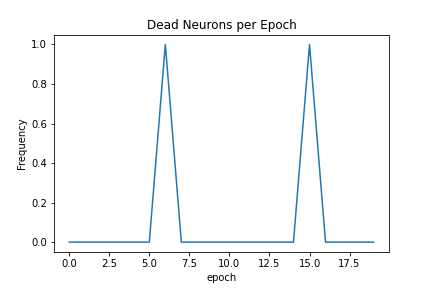
\includegraphics[width=\linewidth]{images/q5/r2/dead.png}
        \caption{تعداد نورون‌های مرده در هر گام}
    \end{subfigure}
    \hfill
    \begin{subfigure}{0.45\linewidth}
        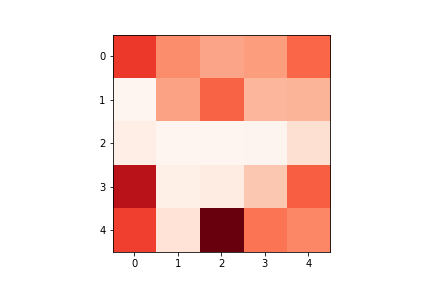
\includegraphics[width=\linewidth]{images/q5/r2/umatrix.png}
        \caption{نمودار \lr{U-Matrix}}
    \end{subfigure}
    \newline
    \begin{subfigure}{0.45\linewidth}
        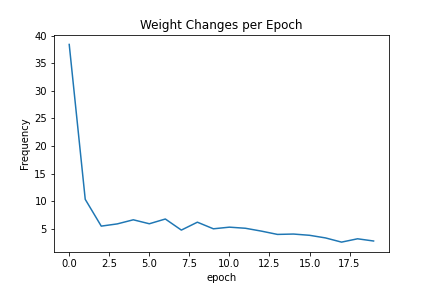
\includegraphics[width=\linewidth]{images/q5/r2/weight_change.png}
        \caption{تغییر وزن‌ها در هر گام}
    \end{subfigure}
    \hfill
    \begin{subfigure}{0.45\linewidth}
        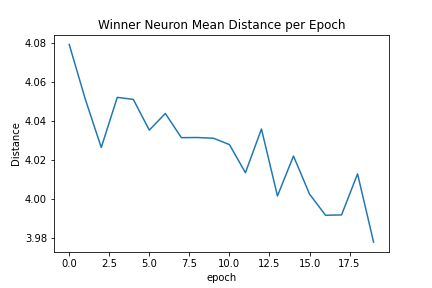
\includegraphics[width=\linewidth]{images/q5/r2/winner_distance.png}
        \caption{فاصله نورون برنده از نورون مدنظر در یک گام}
    \end{subfigure}
    \caption{نمودار‌های آموزش شبکه \lr{SOM} با پارامتر‌های \\$R=2$, $\alpha=0.005$ و ابعاد نقشه $5 \times 5$ با $lr_0=0.1$ و $T=20$}
    \label{r2}
\end{figure}

\clearpage

\begin{figure}[h]
    \begin{subfigure}{\linewidth}
        \centering
        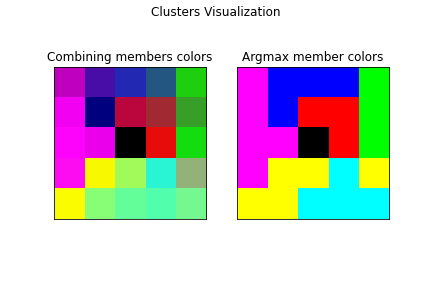
\includegraphics[width=0.8\linewidth]{images/q5/r3/cluster.png}
        \caption{خوشه‌بندی انجام شده توسط شبکه خودسامانده}
    \end{subfigure}
    \newline
    \begin{subfigure}{0.45\linewidth}
        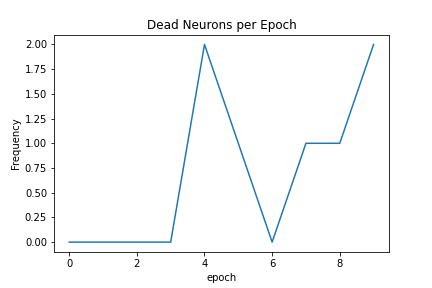
\includegraphics[width=\linewidth]{images/q5/r3/dead.png}
        \caption{تعداد نورون‌های مرده در هر گام}
    \end{subfigure}
    \hfill
    \begin{subfigure}{0.45\linewidth}
        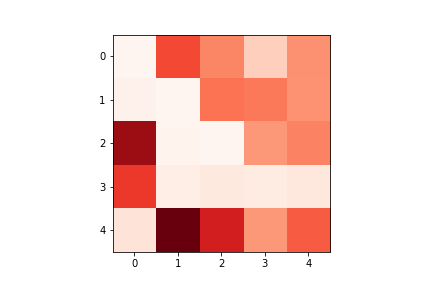
\includegraphics[width=\linewidth]{images/q5/r3/umatrix.png}
        \caption{نمودار \lr{U-Matrix}}
    \end{subfigure}
    \newline
    \begin{subfigure}{0.45\linewidth}
        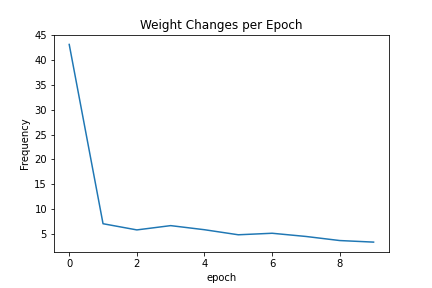
\includegraphics[width=\linewidth]{images/q5/r3/weight_change.png}
        \caption{تغییر وزن‌ها در هر گام}
    \end{subfigure}
    \hfill
    \begin{subfigure}{0.45\linewidth}
        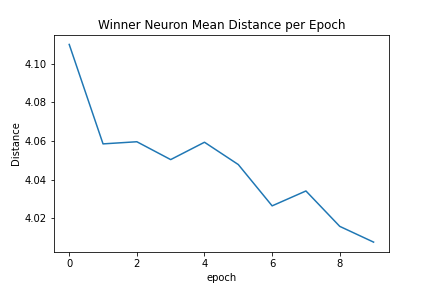
\includegraphics[width=\linewidth]{images/q5/r3/winner_distance.png}
        \caption{فاصله نورون برنده از نورون مدنظر در یک گام}
    \end{subfigure}
    \caption{نمودار‌های آموزش شبکه \lr{SOM} با پارامتر‌های \\$R=2$, $\alpha=0.001$ و ابعاد نقشه $5 \times 5$ با $lr_0=0.1$ و $T=10$}
    \label{r3}
\end{figure}

\clearpage

\begin{figure}[h]
    \begin{subfigure}{\linewidth}
        \centering
        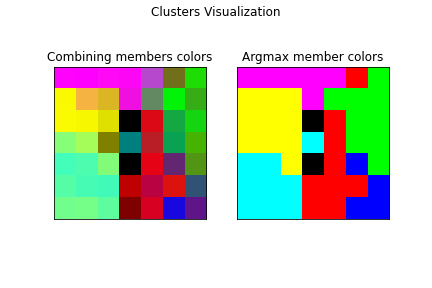
\includegraphics[width=0.8\linewidth]{images/q5/r4/cluster.png}
        \caption{خوشه‌بندی انجام شده توسط شبکه خودسامانده}
    \end{subfigure}
    \newline
    \begin{subfigure}{0.45\linewidth}
        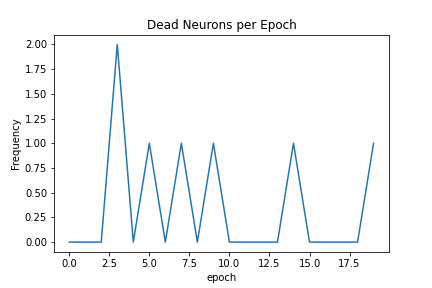
\includegraphics[width=\linewidth]{images/q5/r4/dead.png}
        \caption{تعداد نورون‌های مرده در هر گام}
    \end{subfigure}
    \hfill
    \begin{subfigure}{0.45\linewidth}
        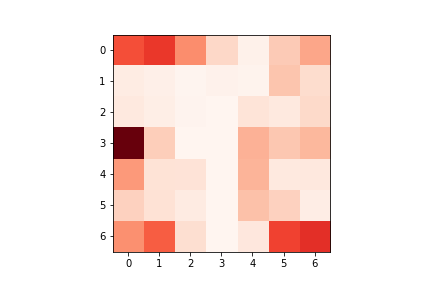
\includegraphics[width=\linewidth]{images/q5/r4/umatrix.png}
        \caption{نمودار \lr{U-Matrix}}
    \end{subfigure}
    \newline
    \begin{subfigure}{0.45\linewidth}
        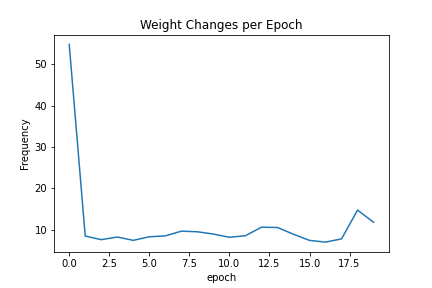
\includegraphics[width=\linewidth]{images/q5/r4/weight_change.png}
        \caption{تغییر وزن‌ها در هر گام}
    \end{subfigure}
    \hfill
    \begin{subfigure}{0.45\linewidth}
        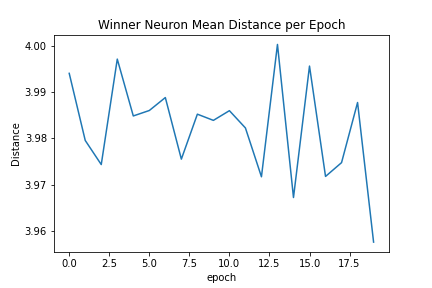
\includegraphics[width=\linewidth]{images/q5/r4/winner_distance.png}
        \caption{فاصله نورون برنده از نورون مدنظر در یک گام}
    \end{subfigure}
    \caption{نمودار‌های آموزش شبکه \lr{SOM} با پارامتر‌های \\$R=3$, $\alpha=0.001$ و ابعاد نقشه $7 \times 7$ با $lr_0=0.1$ و $T=20$}
    \label{r4}
\end{figure}

\clearpage

\begin{figure}[h]
    \begin{subfigure}{\linewidth}
        \centering
        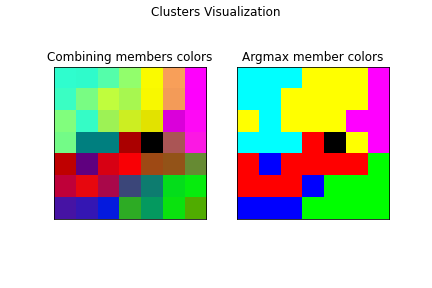
\includegraphics[width=0.8\linewidth]{images/q5/r5/cluster.png}
        \caption{خوشه‌بندی انجام شده توسط شبکه خودسامانده}
    \end{subfigure}
    \newline
    \begin{subfigure}{0.45\linewidth}
        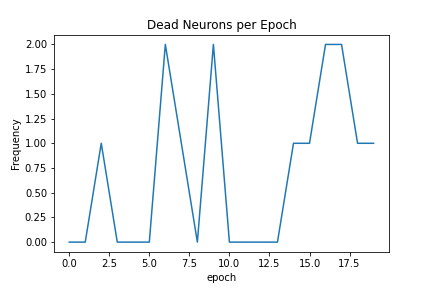
\includegraphics[width=\linewidth]{images/q5/r5/dead.png}
        \caption{تعداد نورون‌های مرده در هر گام}
    \end{subfigure}
    \hfill
    \begin{subfigure}{0.45\linewidth}
        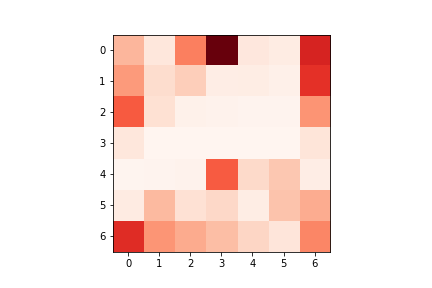
\includegraphics[width=\linewidth]{images/q5/r5/umatrix.png}
        \caption{نمودار \lr{U-Matrix}}
    \end{subfigure}
    \newline
    \begin{subfigure}{0.45\linewidth}
        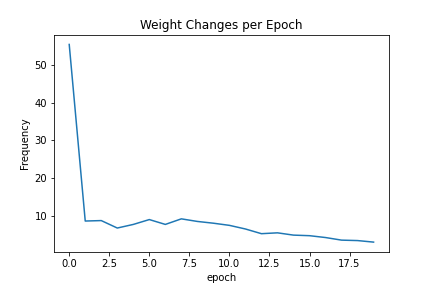
\includegraphics[width=\linewidth]{images/q5/r5/weight_change.png}
        \caption{تغییر وزن‌ها در هر گام}
    \end{subfigure}
    \hfill
    \begin{subfigure}{0.45\linewidth}
        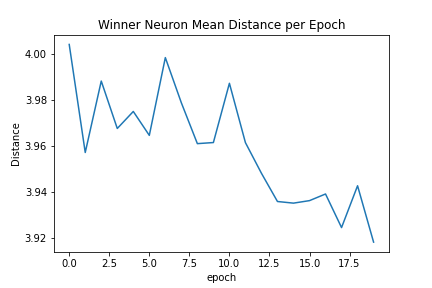
\includegraphics[width=\linewidth]{images/q5/r5/winner_distance.png}
        \caption{فاصله نورون برنده از نورون مدنظر در یک گام}
    \end{subfigure}
    \caption{نمودار‌های آموزش شبکه \lr{SOM} با پارامتر‌های \\$R=3$, $\alpha=0.005$ و ابعاد نقشه $7 \times 7$ با $lr_0=0.1$ و $T=20$}
    \label{r5}
\end{figure}

\clearpage

\begin{figure}[h]
    \begin{subfigure}{\linewidth}
        \centering
        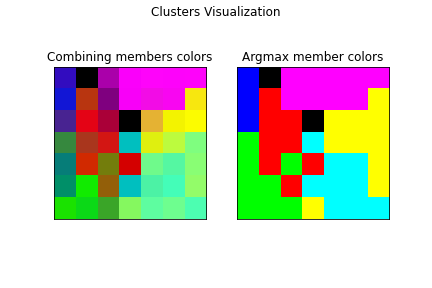
\includegraphics[width=0.8\linewidth]{images/q5/r6/cluster.png}
        \caption{خوشه‌بندی انجام شده توسط شبکه خودسامانده}
    \end{subfigure}
    \newline
    \begin{subfigure}{0.45\linewidth}
        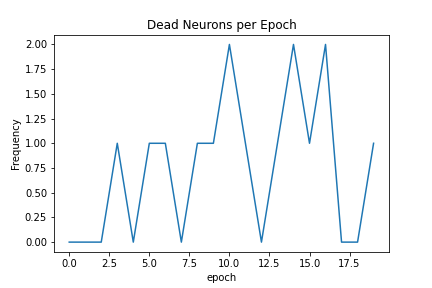
\includegraphics[width=\linewidth]{images/q5/r6/dead.png}
        \caption{تعداد نورون‌های مرده در هر گام}
    \end{subfigure}
    \hfill
    \begin{subfigure}{0.45\linewidth}
        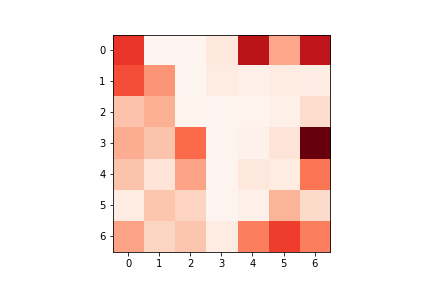
\includegraphics[width=\linewidth]{images/q5/r6/umatrix.png}
        \caption{نمودار \lr{U-Matrix}}
    \end{subfigure}
    \newline
    \begin{subfigure}{0.45\linewidth}
        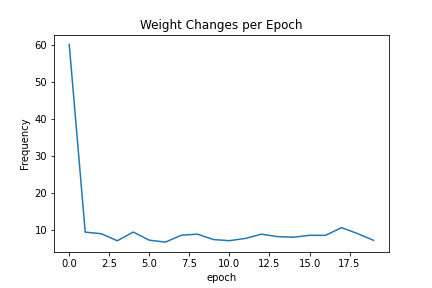
\includegraphics[width=\linewidth]{images/q5/r6/weight_change.png}
        \caption{تغییر وزن‌ها در هر گام}
    \end{subfigure}
    \hfill
    \begin{subfigure}{0.45\linewidth}
        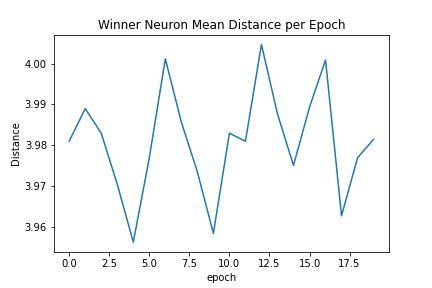
\includegraphics[width=\linewidth]{images/q5/r6/winner_distance.png}
        \caption{فاصله نورون برنده از نورون مدنظر در یک گام}
    \end{subfigure}
    \caption{نمودار‌های آموزش شبکه \lr{SOM} با پارامتر‌های \\$R=3$, $\alpha=0.0001$ و ابعاد نقشه $7 \times 7$ با $lr_0=0.1$ و $T=20$}
    \label{r6}
\end{figure}

\clearpage

\begin{figure}[h]
    \begin{subfigure}{\linewidth}
        \centering
        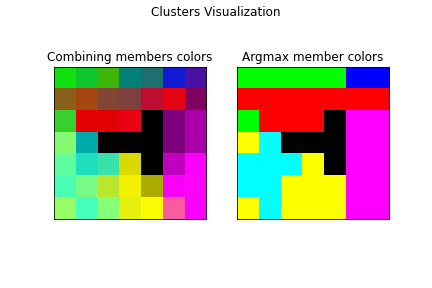
\includegraphics[width=0.8\linewidth]{images/q5/r7/cluster.png}
        \caption{خوشه‌بندی انجام شده توسط شبکه خودسامانده}
    \end{subfigure}
    \newline
    \begin{subfigure}{0.45\linewidth}
        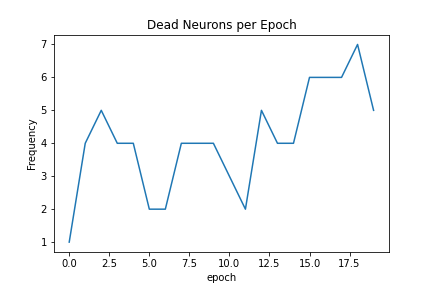
\includegraphics[width=\linewidth]{images/q5/r7/dead.png}
        \caption{تعداد نورون‌های مرده در هر گام}
    \end{subfigure}
    \hfill
    \begin{subfigure}{0.45\linewidth}
        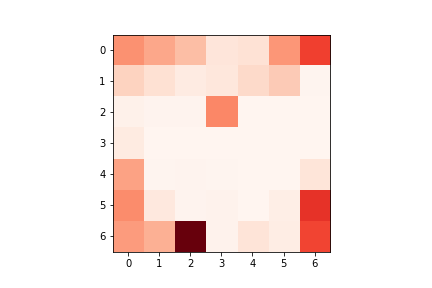
\includegraphics[width=\linewidth]{images/q5/r7/umatrix.png}
        \caption{نمودار \lr{U-Matrix}}
    \end{subfigure}
    \newline
    \begin{subfigure}{0.45\linewidth}
        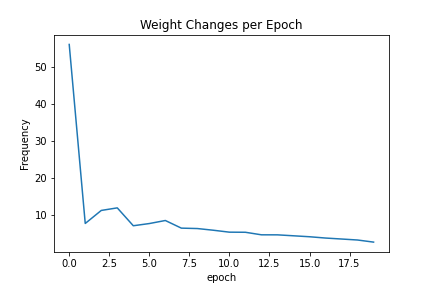
\includegraphics[width=\linewidth]{images/q5/r7/weight_change.png}
        \caption{تغییر وزن‌ها در هر گام}
    \end{subfigure}
    \hfill
    \begin{subfigure}{0.45\linewidth}
        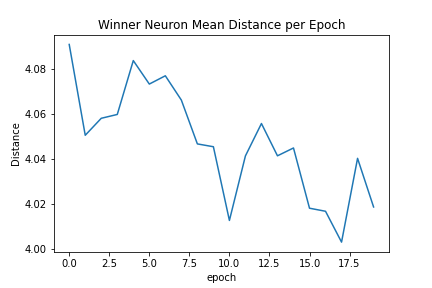
\includegraphics[width=\linewidth]{images/q5/r7/winner_distance.png}
        \caption{فاصله نورون برنده از نورون مدنظر در یک گام}
    \end{subfigure}
    \caption{نمودار‌های آموزش شبکه \lr{SOM} با پارامتر‌های \\$R=4$, $\alpha=0.005$ و ابعاد نقشه $7 \times 7$ با $lr_0=0.1$ و $T=20$}
    \label{r7}
\end{figure}

\clearpage

\begin{figure}[h]
    \begin{subfigure}{\linewidth}
        \centering
        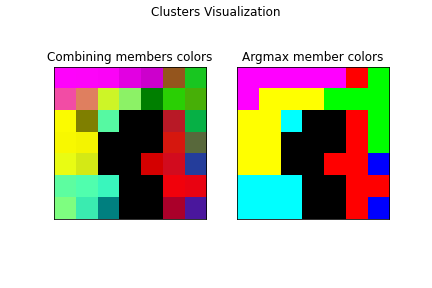
\includegraphics[width=0.8\linewidth]{images/q5/r8/cluster.png}
        \caption{خوشه‌بندی انجام شده توسط شبکه خودسامانده}
    \end{subfigure}
    \newline
    \begin{subfigure}{0.45\linewidth}
        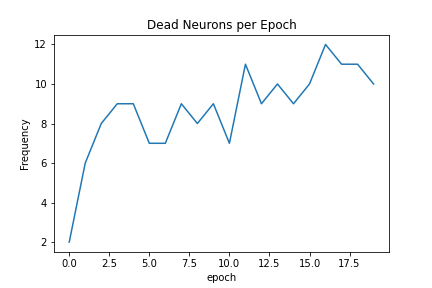
\includegraphics[width=\linewidth]{images/q5/r8/dead.png}
        \caption{تعداد نورون‌های مرده در هر گام}
    \end{subfigure}
    \hfill
    \begin{subfigure}{0.45\linewidth}
        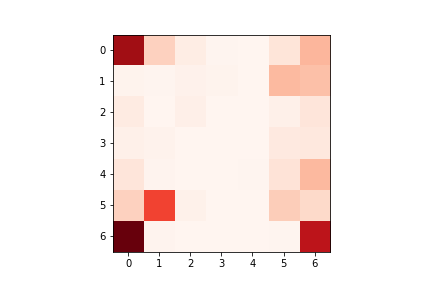
\includegraphics[width=\linewidth]{images/q5/r8/umatrix.png}
        \caption{نمودار \lr{U-Matrix}}
    \end{subfigure}
    \newline
    \begin{subfigure}{0.45\linewidth}
        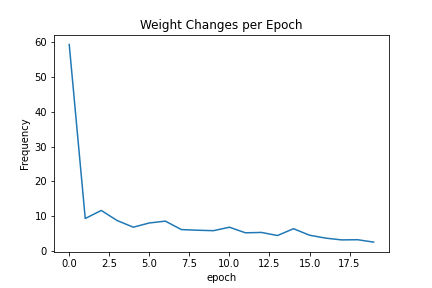
\includegraphics[width=\linewidth]{images/q5/r8/weight_change.png}
        \caption{تغییر وزن‌ها در هر گام}
    \end{subfigure}
    \hfill
    \begin{subfigure}{0.45\linewidth}
        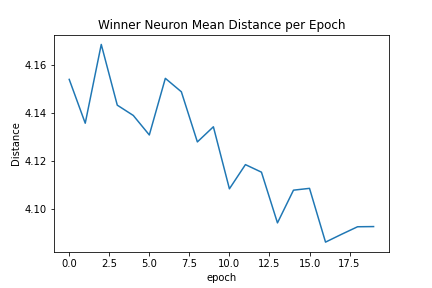
\includegraphics[width=\linewidth]{images/q5/r8/winner_distance.png}
        \caption{فاصله نورون برنده از نورون مدنظر در یک گام}
    \end{subfigure}
    \caption{نمودار‌های آموزش شبکه \lr{SOM} با پارامتر‌های \\$R=5$, $\alpha=0.005$ و ابعاد نقشه $7 \times 7$ با $lr_0=0.1$ و $T=20$}
    \label{r8}
\end{figure}

\clearpage

\begin{figure}[h]
    \begin{subfigure}{\linewidth}
        \centering
        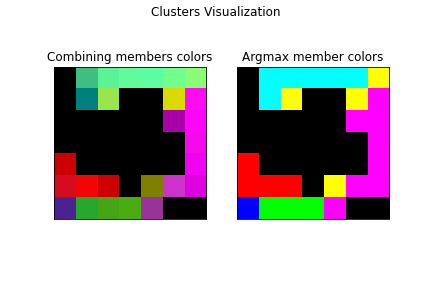
\includegraphics[width=0.8\linewidth]{images/q5/r9/cluster.png}
        \caption{خوشه‌بندی انجام شده توسط شبکه خودسامانده}
    \end{subfigure}
    \newline
    \begin{subfigure}{0.45\linewidth}
        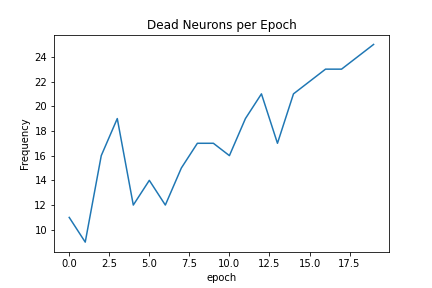
\includegraphics[width=\linewidth]{images/q5/r9/dead.png}
        \caption{تعداد نورون‌های مرده در هر گام}
    \end{subfigure}
    \hfill
    \begin{subfigure}{0.45\linewidth}
        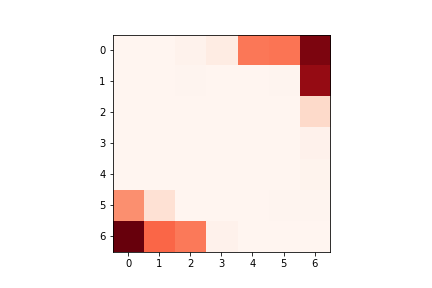
\includegraphics[width=\linewidth]{images/q5/r9/umatrix.png}
        \caption{نمودار \lr{U-Matrix}}
    \end{subfigure}
    \newline
    \begin{subfigure}{0.45\linewidth}
        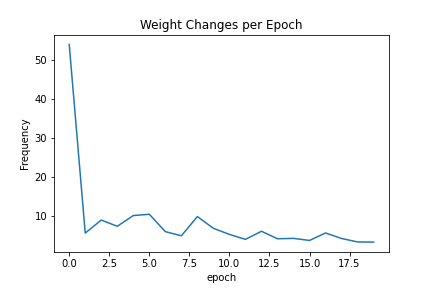
\includegraphics[width=\linewidth]{images/q5/r9/weight_change.png}
        \caption{تغییر وزن‌ها در هر گام}
    \end{subfigure}
    \hfill
    \begin{subfigure}{0.45\linewidth}
        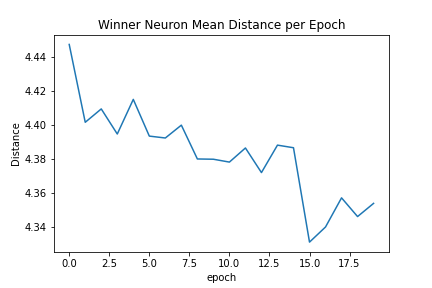
\includegraphics[width=\linewidth]{images/q5/r9/winner_distance.png}
        \caption{فاصله نورون برنده از نورون مدنظر در یک گام}
    \end{subfigure}
    \caption{نمودار‌های آموزش شبکه \lr{SOM} با پارامتر‌های \\$R=7$, $\alpha=0.005$ و ابعاد نقشه $7 \times 7$ با $lr_0=0.1$ و $T=20$}
    \label{r9}
\end{figure}

\begin{figure}[h]
    \begin{subfigure}{\linewidth}
        \centering
        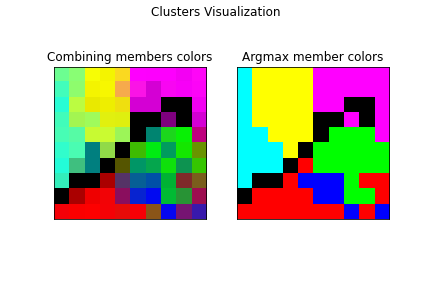
\includegraphics[width=0.8\linewidth]{images/q5/r10/cluster.png}
        \caption{خوشه‌بندی انجام شده توسط شبکه خودسامانده}
    \end{subfigure}
    \newline
    \begin{subfigure}{0.45\linewidth}
        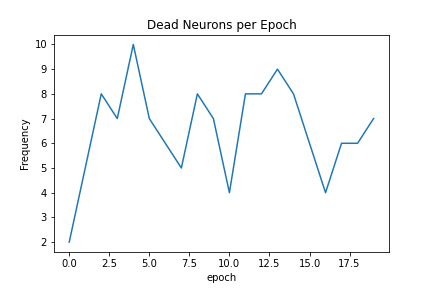
\includegraphics[width=\linewidth]{images/q5/r10/dead.png}
        \caption{تعداد نورون‌های مرده در هر گام}
    \end{subfigure}
    \hfill
    \begin{subfigure}{0.45\linewidth}
        \includegraphics[width=\linewidth]{images/q5/r10/umatrix.png}
        \caption{نمودار \lr{U-Matrix}}
    \end{subfigure}
    \newline
    \begin{subfigure}{0.45\linewidth}
        \includegraphics[width=\linewidth]{images/q5/r10/weight_change.png}
        \caption{تغییر وزن‌ها در هر گام}
    \end{subfigure}
    \hfill
    \begin{subfigure}{0.45\linewidth}
        \includegraphics[width=\linewidth]{images/q5/r10/winner_distance.png}
        \caption{فاصله نورون برنده از نورون مدنظر در یک گام}
    \end{subfigure}
    \caption{نمودار‌های آموزش شبکه \lr{SOM} با پارامتر‌های \\$R=4$, $\alpha=0.00001$ و ابعاد نقشه $10 \times 10$ با $lr_0=0.1$ و $T=20$}
    \label{r10}
\end{figure}

\clearpage

\begin{figure}[h]
    \begin{subfigure}{\linewidth}
        \centering
        \includegraphics[width=0.8\linewidth]{images/q5/r11/cluster.png}
        \caption{خوشه‌بندی انجام شده توسط شبکه خودسامانده}
    \end{subfigure}
    \newline
    \begin{subfigure}{0.45\linewidth}
        \includegraphics[width=\linewidth]{images/q5/r11/dead.png}
        \caption{تعداد نورون‌های مرده در هر گام}
    \end{subfigure}
    \hfill
    \begin{subfigure}{0.45\linewidth}
        \includegraphics[width=\linewidth]{images/q5/r11/umatrix.png}
        \caption{نمودار \lr{U-Matrix}}
    \end{subfigure}
    \newline
    \begin{subfigure}{0.45\linewidth}
        \includegraphics[width=\linewidth]{images/q5/r11/weight_change.png}
        \caption{تغییر وزن‌ها در هر گام}
    \end{subfigure}
    \hfill
    \begin{subfigure}{0.45\linewidth}
        \includegraphics[width=\linewidth]{images/q5/r11/winner_distance.png}
        \caption{فاصله نورون برنده از نورون مدنظر در یک گام}
    \end{subfigure}
    \caption{نمودار‌های آموزش شبکه \lr{SOM} با پارامتر‌های \\$R=4$, $\alpha=0.0001$ و ابعاد نقشه $10 \times 10$ با $lr_0=0.1$ و $T=20$}
    \label{r11}
\end{figure}

\clearpage

\begin{figure}[h]
    \begin{subfigure}{\linewidth}
        \centering
        \includegraphics[width=0.8\linewidth]{images/q5/r12/cluster.png}
        \caption{خوشه‌بندی انجام شده توسط شبکه خودسامانده}
    \end{subfigure}
    \newline
    \begin{subfigure}{0.45\linewidth}
        \includegraphics[width=\linewidth]{images/q5/r12/dead.png}
        \caption{تعداد نورون‌های مرده در هر گام}
    \end{subfigure}
    \hfill
    \begin{subfigure}{0.45\linewidth}
        \includegraphics[width=\linewidth]{images/q5/r12/umatrix.png}
        \caption{نمودار \lr{U-Matrix}}
    \end{subfigure}
    \newline
    \begin{subfigure}{0.45\linewidth}
        \includegraphics[width=\linewidth]{images/q5/r12/weight_change.png}
        \caption{تغییر وزن‌ها در هر گام}
    \end{subfigure}
    \hfill
    \begin{subfigure}{0.45\linewidth}
        \includegraphics[width=\linewidth]{images/q5/r12/winner_distance.png}
        \caption{فاصله نورون برنده از نورون مدنظر در یک گام}
    \end{subfigure}
    \caption{نمودار‌های آموزش شبکه \lr{SOM} با پارامتر‌های \\$R=4$, $\alpha=0.005$ و ابعاد نقشه $10 \times 10$ با $lr_0=0.1$ و $T=20$}
    \label{r12}
\end{figure}

\clearpage

\begin{figure}[h]
    \begin{subfigure}{\linewidth}
        \centering
        \includegraphics[width=0.8\linewidth]{images/q5/r13/cluster.png}
        \caption{خوشه‌بندی انجام شده توسط شبکه خودسامانده}
    \end{subfigure}
    \newline
    \begin{subfigure}{0.45\linewidth}
        \includegraphics[width=\linewidth]{images/q5/r13/dead.png}
        \caption{تعداد نورون‌های مرده در هر گام}
    \end{subfigure}
    \hfill
    \begin{subfigure}{0.45\linewidth}
        \includegraphics[width=\linewidth]{images/q5/r13/umatrix.png}
        \caption{نمودار \lr{U-Matrix}}
    \end{subfigure}
    \newline
    \begin{subfigure}{0.45\linewidth}
        \includegraphics[width=\linewidth]{images/q5/r13/weight_change.png}
        \caption{تغییر وزن‌ها در هر گام}
    \end{subfigure}
    \hfill
    \begin{subfigure}{0.45\linewidth}
        \includegraphics[width=\linewidth]{images/q5/r13/winner_distance.png}
        \caption{فاصله نورون برنده از نورون مدنظر در یک گام}
    \end{subfigure}
    \caption{نمودار‌های آموزش شبکه \lr{SOM} با پارامتر‌های \\$R=5$, $\alpha=0.005$ و ابعاد نقشه $10 \times 10$ با $lr_0=0.1$ و $T=20$}
    \label{r13}
\end{figure}

\clearpage

\begin{figure}[h]
    \begin{subfigure}{\linewidth}
        \centering
        \includegraphics[width=0.8\linewidth]{images/q5/r14/cluster.png}
        \caption{خوشه‌بندی انجام شده توسط شبکه خودسامانده}
    \end{subfigure}
    \newline
    \begin{subfigure}{0.45\linewidth}
        \includegraphics[width=\linewidth]{images/q5/r14/dead.png}
        \caption{تعداد نورون‌های مرده در هر گام}
    \end{subfigure}
    \hfill
    \begin{subfigure}{0.45\linewidth}
        \includegraphics[width=\linewidth]{images/q5/r14/umatrix.png}
        \caption{نمودار \lr{U-Matrix}}
    \end{subfigure}
    \newline
    \begin{subfigure}{0.45\linewidth}
        \includegraphics[width=\linewidth]{images/q5/r14/weight_change.png}
        \caption{تغییر وزن‌ها در هر گام}
    \end{subfigure}
    \hfill
    \begin{subfigure}{0.45\linewidth}
        \includegraphics[width=\linewidth]{images/q5/r14/winner_distance.png}
        \caption{فاصله نورون برنده از نورون مدنظر در یک گام}
    \end{subfigure}
    \caption{نمودار‌های آموزش شبکه \lr{SOM} با پارامتر‌های \\$R=7$, $\alpha=0.005$ و ابعاد نقشه $10 \times 10$ با $lr_0=0.1$ و $T=20$}
    \label{r14}
\end{figure}

\clearpage

\begin{figure}[h]
    \begin{subfigure}{\linewidth}
        \centering
        \includegraphics[width=0.8\linewidth]{images/q5/r15/cluster.png}
        \caption{خوشه‌بندی انجام شده توسط شبکه خودسامانده}
    \end{subfigure}
    \newline
    \begin{subfigure}{0.45\linewidth}
        \includegraphics[width=\linewidth]{images/q5/r15/dead.png}
        \caption{تعداد نورون‌های مرده در هر گام}
    \end{subfigure}
    \hfill
    \begin{subfigure}{0.45\linewidth}
        \includegraphics[width=\linewidth]{images/q5/r15/umatrix.png}
        \caption{نمودار \lr{U-Matrix}}
    \end{subfigure}
    \newline
    \begin{subfigure}{0.45\linewidth}
        \includegraphics[width=\linewidth]{images/q5/r15/weight_change.png}
        \caption{تغییر وزن‌ها در هر گام}
    \end{subfigure}
    \hfill
    \begin{subfigure}{0.45\linewidth}
        \includegraphics[width=\linewidth]{images/q5/r15/winner_distance.png}
        \caption{فاصله نورون برنده از نورون مدنظر در یک گام}
    \end{subfigure}
    \caption{نمودار‌های آموزش شبکه \lr{SOM} با پارامتر‌های \\$R=3$, $\alpha=0.005$ و ابعاد نقشه $13 \times 13$ با $lr_0=0.1$ و $T=20$}
    \label{r15}
\end{figure}

\clearpage

\begin{figure}[h]
    \begin{subfigure}{\linewidth}
        \centering
        \includegraphics[width=0.8\linewidth]{images/q5/r16/cluster.png}
        \caption{خوشه‌بندی انجام شده توسط شبکه خودسامانده}
    \end{subfigure}
    \newline
    \begin{subfigure}{0.45\linewidth}
        \includegraphics[width=\linewidth]{images/q5/r16/dead.png}
        \caption{تعداد نورون‌های مرده در هر گام}
    \end{subfigure}
    \hfill
    \begin{subfigure}{0.45\linewidth}
        \includegraphics[width=\linewidth]{images/q5/r16/umatrix.png}
        \caption{نمودار \lr{U-Matrix}}
    \end{subfigure}
    \newline
    \begin{subfigure}{0.45\linewidth}
        \includegraphics[width=\linewidth]{images/q5/r16/weight_change.png}
        \caption{تغییر وزن‌ها در هر گام}
    \end{subfigure}
    \hfill
    \begin{subfigure}{0.45\linewidth}
        \includegraphics[width=\linewidth]{images/q5/r16/winner_distance.png}
        \caption{فاصله نورون برنده از نورون مدنظر در یک گام}
    \end{subfigure}
    \caption{نمودار‌های آموزش شبکه \lr{SOM} با پارامتر‌های \\$R=5$, $\alpha=0.005$ و ابعاد نقشه $13 \times 13$ با $lr_0=0.1$ و $T=20$}
    \label{r16}
\end{figure}

\clearpage

\begin{figure}[h]
    \begin{subfigure}{\linewidth}
        \centering
        \includegraphics[width=0.8\linewidth]{images/q5/r17/cluster.png}
        \caption{خوشه‌بندی انجام شده توسط شبکه خودسامانده}
    \end{subfigure}
    \newline
    \begin{subfigure}{0.45\linewidth}
        \includegraphics[width=\linewidth]{images/q5/r17/dead.png}
        \caption{تعداد نورون‌های مرده در هر گام}
    \end{subfigure}
    \hfill
    \begin{subfigure}{0.45\linewidth}
        \includegraphics[width=\linewidth]{images/q5/r17/umatrix.png}
        \caption{نمودار \lr{U-Matrix}}
    \end{subfigure}
    \newline
    \begin{subfigure}{0.45\linewidth}
        \includegraphics[width=\linewidth]{images/q5/r17/weight_change.png}
        \caption{تغییر وزن‌ها در هر گام}
    \end{subfigure}
    \hfill
    \begin{subfigure}{0.45\linewidth}
        \includegraphics[width=\linewidth]{images/q5/r17/winner_distance.png}
        \caption{فاصله نورون برنده از نورون مدنظر در یک گام}
    \end{subfigure}
    \caption{نمودار‌های آموزش شبکه \lr{SOM} با پارامتر‌های \\$R=7$, $\alpha=0.005$ و ابعاد نقشه $13 \times 13$ با $lr_0=0.1$ و $T=20$}
    \label{r17}
\end{figure}

\clearpage

\begin{figure}[h]
    \begin{subfigure}{\linewidth}
        \centering
        \includegraphics[width=0.8\linewidth]{images/q5/r18/cluster.png}
        \caption{خوشه‌بندی انجام شده توسط شبکه خودسامانده}
    \end{subfigure}
    \newline
    \begin{subfigure}{0.45\linewidth}
        \includegraphics[width=\linewidth]{images/q5/r18/dead.png}
        \caption{تعداد نورون‌های مرده در هر گام}
    \end{subfigure}
    \hfill
    \begin{subfigure}{0.45\linewidth}
        \includegraphics[width=\linewidth]{images/q5/r18/umatrix.png}
        \caption{نمودار \lr{U-Matrix}}
    \end{subfigure}
    \newline
    \begin{subfigure}{0.45\linewidth}
        \includegraphics[width=\linewidth]{images/q5/r18/weight_change.png}
        \caption{تغییر وزن‌ها در هر گام}
    \end{subfigure}
    \hfill
    \begin{subfigure}{0.45\linewidth}
        \includegraphics[width=\linewidth]{images/q5/r18/winner_distance.png}
        \caption{فاصله نورون برنده از نورون مدنظر در یک گام}
    \end{subfigure}
    \caption{نمودار‌های آموزش شبکه \lr{SOM} با پارامتر‌های \\$R=9$, $\alpha=0.005$ و ابعاد نقشه $13 \times 13$ با $lr_0=0.1$ و $T=20$}
    \label{r18}
\end{figure}

\clearpage

\section*{سوال ششم}

برای کاهش ابعاد داده‌ها از دو روش استفاده می‌کنیم. در روش اول فاصله هر داده تا هر نورون خروجی را محاسبه کرده
و بردار حاصل از این مقادیر را به شبکه عصبی می‌دهیم. در این حالت داده اگر تعداد نورون موجود در لایه خروجی
برابر ۱۰۰ باشد داده به فضای ۱۰۰ بعدی نگاشت می‌شود. در روش دوم هر داده ورودی با استفاده از ایندکس نزدیک‌ترین نورون
ورودی به آن نمایش داده می‌شود. بدین ترتیب اگر نورون شماره $(2,5)$ در صفحه خروجی $10 \times 10$ نزدیک‌ترین نورون
به بردار ورودی باشد، داده با زوج $(2,5)$ نشان داده می‌شود. در این حالت بردار ورودی به یک فضای دو بعدی نگاشت می‌شود.

در ادامه عملکرد شبکه در هنگام کاهش ابعاد با استفاده از روش فاصله تا هر نورون بررسی می‌شود.
برای این حالت شبکه را با تعداد مختلف لایه‌های پنهان و تعداد نورون‌های مختلف در هر لایه بررسی می‌کنیم.
لازم به ذکر است در حین این کار ما نرخ یادگیری شبکه را برابر $0.0001$ قرار داده‌ایم.
همان‌طور که در جدول زیر مشاهده می‌شود، با افزایش تعداد لایه‌های پنهان و تعداد نورون‌ها در لایه پنهان عملکرد شبکه
رفته‌رفته بهتر می‌شود. از بین حالت‌های بررسی شده شبکه با یک لایه مخفی که تعداد ۸۱۹۲ نورون دارد،
بهترین عملکرد را ارائه داده است، بنابراین در ادامه از شبکه با این ساختار استفاده خواهیم کرد.
در جدول بعدی تاثیر نرخ یادگیری بر روی عملکرد مدل انتخابی آورده شده است، همان‌طور که مشاهده می‌شود
شبکه به ازای نرخ یادگیری $0.0001$ بهترین عملکرد را داراست. با این پارامتر‌ها، مدل بر روی داده‌های آزمون
می‌تواند به صحت $0.7503$ و خطای $0.5663$ برسد.

\begin{latin}
\begin{table}[!ht]
    \centering
    \caption{\rl{آزمون خطاهای انجام شده برای یافتن بهترین تعداد لایه پنهان و نورون‌ موجود در هر لایه}}
    \begin{tabular}{|l|l|c|c|c|c|}
    \hline
        & & \multicolumn{2}{c|}{train} & \multicolumn{2}{c|}{validation}  \\ \hline
        index & hidden layer & accuracy & loss & accuracy & loss \\ \hline
        1 & - & 0.7273 & 0.6305 & 0.7866 & 0.6374 \\ \hline
        2 & (16,) & 0.4916 & 0.9919 & 0.5548 & 0.9729 \\ \hline
        3 & (32,) & 0.6831 & 0.7569 & 0.6848 & 0.7709 \\ \hline
        4 & (512,) & 0.7718 & 0.5593 & 0.7939 & 0.5747 \\ \hline
        5 & (4096,) & 0.7748 & 0.5065 & 0.8099 & 0.5111 \\ \hline
        6 & (8192,) & 0.7893 & 0.489 & 0.7973 & 0.48 \\ \hline
        7 & (8192, 8192) & 0.7707 & 0.504 & 0.7696 & 0.5066 \\ \hline
        8 & (8192, 8192, 8192) & 0.7686 & 0.507 & 0.7866 & 0.4813 \\ \hline
        9 & (4096, 4096, 4096, 4096) & 0.7709 & 0.4925 & 0.7556 & 0.5627 \\ \hline
        10 & (4096, 4096, 4096, 4096, 4096) & 0.7655 & 0.5023 & 0.7401 & 0.5016 \\ \hline
    \end{tabular}
\end{table}
\end{latin}

\begin{latin}
\begin{table}[!ht]
    \centering
    \caption{\rl{آزمون خطاهای انجام شده برای یافتن بهترین نرخ یادگیری}}
    \begin{tabular}{|l|l|c|c|c|c|}
    \hline
        & & \multicolumn{2}{c|}{train} & \multicolumn{2}{c|}{validation}  \\ \hline
        index & learning rate & accuracy & loss & accuracy & loss \\ \hline
        1 & 1.00E-06 & 0.6642 & 0.9381 & 0.7056 & 0.9394 \\ \hline
        2 & 1.00E-05 & 0.727 & 0.6395 & 0.7687 & 0.6386 \\ \hline
        3 & 0.0001 & 0.7771 & 0.5009 & 0.709 & 0.5681 \\ \hline
        4 & 0.001 & 0.769 & 0.498 & 0.7541 & 0.4981 \\ \hline
        5 & 0.01 & 0.1914 & 1.7844 & 0.1765 & 1.7903 \\ \hline
        6 & 0.1 & 0.1767 & 1.7895 & 0.1857 & 1.7936 \\ \hline
    \end{tabular}
\end{table}
\end{latin}

\newpage

برخلاف انتظار ما اعمال کاهش بعد در داده‌ نه تنها باعث بهبود عملکرد مدل شبکه عصبی نشد بلکه عملکرد آن‌ را کاهش داده است.
افت عملکرد شبکه عصبی طبیعی به نظر می‌رسد چرا که طبق شکل \ref{r17} شبکه \lr{SOM} نتوانسته‌ است داده‌های یک دسته
را به خوبی از دیگر داده‌ها تمییز دهد. در نتیجه قابل انتظار است که شبکه نتواند بین داده‌های یک دسته تمییز قائل شود.
البته خود عمل کاهش بعد مزیت‌هایی نیز ایجاد می‌کند. مثلا با کاهش ابعاد بعد ورودی داده کوچک‌تر شده و در نتیجه اتصالات لایه
اول به لایه‌ مخفی اول کم‌تر می‌شود. این قسمت، هر چند اندک، اما می‌تواند سرعت شبکه را افزایش دهد. برای بهبود عملکرد شبکه
\lr{SOM} به نظر می‌رسد که باید شعاع اثر داده برنده را در طی زمان کاهش دهیم تا شبکه بتواند داده‌های متناظر
یک خوشه را به خوبی از دیگری جدا کند.

حال عملکرد شبکه عصبی را در هنگام کاهش ابعاد با استفاده از ایندکس نورون برنده را بررسی می‌کنیم. ابتدا تلاش می‌کنیم
ساختار بهینه شبکه عصبی را پیدا کنیم. این کار را با تغییر تعداد نورون‌های موجود در هر لایه و تغییر تعداد لایه‌ها
انجام می‌دهیم. در جدول زیر سعی و خطاهای انجام شده برای یافتن بهترین مقدار برای این دو پارامتر آورده شده است.
لازم به ذکر است که برای یافتن این پارامتر‌ها نرخ یادگیری مدل برابر $0.0001$ در نظر گرفته شده بود. همان‌طور که در
جدول قابل مشاهده است، شبکه در هنگامی که سه لایه پنهان با تعداد ۴۰۹۶ نورون دارد بهترین عملکرد را از خود نشان می‌دهد.
با توجه به جدول زیر با تغییر نرخ یادگیری مدل به مقادیر کوچک‌تر و بزرگ‌تر نتیجه بهتری حاصل نشده و
مدل به ازای نرخ یادگیری $0.0001$ بهترین عملکرد را داراست. با ارزیابی مدل بر روی داده‌های آزمون،
مدل صحت $0.6994$ و خطای $0.5487$ را ارائه می‌دهد که در مقایسه با حالت قبلی کم‌تر است.

\begin{latin}
\begin{table}[!ht]
    \centering
    \caption{\rl{آزمون خطاهای انجام شده برای یافتن بهترین تعداد لایه پنهان و نورون‌ موجود در هر لایه}}
    \begin{tabular}{|l|l|c|c|c|c|}
    \hline
        & & \multicolumn{2}{c|}{train} & \multicolumn{2}{c|}{validation}  \\ \hline
        index & hidden layer & accuracy & loss & accuracy & loss \\ \hline
        1 & - & 0.5710 & 0.9599 & 0.5679 & 0.9924 \\ \hline
        2 & (16,) & 0.4962 & 1.2182 & 0.4738 & 1.2572 \\ \hline
        3 & (32,) & 0.962 & 0.6038 & 0.6004 & 0.9955 \\ \hline
        4 & (512,) & 0.7978 & 0.6736 & 0.6552 & 0.8506 \\ \hline
        5 & (4096,) & 0.7856 & 0.6359 & 0.7449 & 0.6802 \\ \hline
        6 & (8192,) & 0.7829 & 0.6001 & 0.7915 & 0.6409 \\ \hline
        7 & (4096, 4096) & 0.7818 & 0.4932 & 0.7939 & 0.5178 \\ \hline
        8 & (4096, 4096, 4096) & 0.7983 & 0.4683 & 0.8046 & 0.5119 \\ \hline
        9 & (4096, 4096, 4096, 4096) & 0.7937 & 0.4649 & 0.7949 & 0.5169 \\ \hline
        10 & (4096, 4096, 4096, 4096, 4096) & 0.7941 & 0.4686 & 0.7658 & 0.5391 \\ \hline
    \end{tabular}
\end{table}
\end{latin}

\begin{latin}
\begin{table}[!ht]
    \centering
    \caption{\rl{آزمون خطاهای انجام شده برای یافتن بهترین نرخ یادگیری}}
    \begin{tabular}{|l|l|c|c|c|c|}
    \hline
        & & \multicolumn{2}{c|}{train} & \multicolumn{2}{c|}{validation}  \\ \hline
        index & learning rate & accuracy & loss & accuracy & loss \\ \hline
        1 & 1.00E-06 & 0.5517 & 1.1189 & 0.5533 & 1.1401 \\ \hline
        2 & 1.00E-05 & 0.6477 & 0.7946 & 0.6363 & 0.86 \\ \hline
        3 & 0.0001 & 0.7786 & 0.4866 & 0.7726 & 0.5418 \\ \hline
        4 & 0.001 & 0.7908 & 0.467 & 0.7726 & 0.5185 \\ \hline
        5 & 0.01 & 0.7693 & 0.4993 & 0.7823 & 0.5264 \\ \hline
        6 & 0.1 & 0.1914 & 1.784 & 0.1765 & 1.7906 \\ \hline
    \end{tabular}
\end{table}
\end{latin}

\newpage

همان‌طور که مشاهده می‌شود خوشه‌بندی \lr{SOM} در این حالت نیز نتوانسته است عملکرد شبکه عصبی را بهبود ببخشد.
البته این موضوع نیز با توجه به توضیحاتی که پیش‌تر دادیم منطقی به نظر می‌رسد. حتی می‌توان بیان کرد که \lr{SOM} در این حالت
از عملکرد بهترین برخوردار است چرا که با کاهش ابعاد داده‌ها به دو بعد توانسته‌ است به دقت $0.7908$ برسد،
که در مقایسه با حالت قبلی که داده‌ها به فضای 169 بعدی نگاشت شده بود عملکرد بسیار بهتر است.

\end{document}